%! TeX program = lualatex
\documentclass[12pt]{article}

\usepackage{cmap}
\usepackage{tabularx}
\usepackage[newfloat]{minted}
\usepackage[font=small]{caption}
\usepackage{indentfirst}
\usepackage{booktabs} % \toprule, \midrule, \bottomrule
\usepackage[table]{xcolor}

\usepackage{tikz}
\usetikzlibrary{shapes, arrows.meta, positioning, shadows}

\setminted{
    linenos,                % показывать номера строк
    breaklines,             % переносить длинные строки
    breakanywhere=true,     % переносить в любом месте
    tabsize=2,              % размер табуляции
    fontsize=\footnotesize,        % размер шрифта
    frame=lines,            % рамка сверху и снизу
    framesep=2mm,           % расстояние текста от рамки
    baselinestretch=1.1,    % межстрочный интервал
    autogobble=true,        % автоудаление общего отступа
    % xleftmargin=10pt,       % отступ слева
    % numbersep=5pt,          % расстояние между номерами и кодом
}

\usepackage[english, russian]{babel}

\usepackage[nopatch=footnote]{microtype}

\usepackage{float}
\usepackage{fontspec}

\usepackage{enumitem}

\makeatletter
\renewcommand\@seccntformat[1]{%
  \csname the#1\endcsname.\quad
}
\makeatother

\usepackage{tocloft}
\renewcommand{\cftsecaftersnum}{.}
\renewcommand{\cftsubsecaftersnum}{.}
\renewcommand{\cftsubsubsecaftersnum}{.}

\renewcommand{\cftsecleader}{\cftdotfill{\cftdotsep}}

\usepackage[pdfborder={0 0 0}]{hyperref}
\usepackage{subfig}
\usepackage{newfloat}

\setmainfont{TimesNewerRoman}[
  Extension = .otf,
  Path = /nix/store/ihdqrn4p54awd89vrday9k53s8i47bbv-times-newer-roman-unstable-2018-09-11/share/fonts/opentype/,
  UprightFont = *-Regular,
  BoldFont = *-Bold,
  ItalicFont = *-Italic
]

\setmonofont{Ubuntu Mono}

\newcommand{\icon}[1]{\fontspec{UbuntuNerdFont}[Extension = .ttf,
  Path = /nix/store/h721jafy2n74x4k5p0hxbz722h0rncmx-nerd-fonts-ubuntu-3.3.0+0.83/share/fonts/truetype/NerdFonts/Ubuntu/,
  UprightFont = *-Regular,
BoldFont = *-Bold] #1}

\newcommand{\iicon}[1]{{\icon{#1}}}

\usepackage{graphicx}
\usepackage{fontawesome5} % Для иконок

\usepackage[left=2.0cm, right=2.0cm, top=1.0cm, bottom=1.0cm, includeheadfoot]{geometry}

% \usepackage[mocha, textcolor=true, pagecolor=true]{catppuccinpalette} \usemintedstyle{catppuccin-mocha}
\usepackage[latte, textcolor=true, pagecolor=true]{catppuccinpalette} \usemintedstyle{catppuccin-latte}

\usepackage{setspace}
\onehalfspacing

\usepackage{fancyhdr}
\fancyhf{}

\renewcommand{\sectionmark}[1]{\markboth{#1}{}}
\renewcommand{\subsectionmark}[1]{\markright{#1}}

% Настройка колонтитулов
\fancyhead[RO]{\rightmark}
\fancyhead[LO]{\leftmark}

\fancyfoot[L]{\hspace{8pt} \rule{\textwidth}{0.4pt}}
\fancyfoot[R]{\LARGE{\thepage}}
\fancyfoot[C]{}

\newcommand{\lablogo}
{
\begin{center}
    \huge{\textbf{Лабораторная работа №2}} \\
\end{center}
}

\newcommand{\colorURL}[1]{\textcolor{CtpBlue}{#1}}
\newcommand{\colorGIT}[1]{\textcolor{CtpLavender}{#1}}
\renewcommand{\texttt}[1]{{\small\ttfamily #1}}

\setlength{\headheight}{15.2pt}

\DeclareCaptionLabelFormat{gostfigure}{Рисунок #2}
\captionsetup[figure]{labelformat=gostfigure, labelsep=endash}

% \DeclareCaptionLabelFormat{gostfigure}{Таблица #2}
% \captionsetup[table]{labelformat=gostfigure, labelsep=endash}

\DeclareCaptionLabelFormat{gostlisting}{Листинг #2}
\newenvironment{code}
  {\par\captionsetup{type=listing}\noindent}
  {\par\vspace{\baselineskip}}
\captionsetup[listing]{labelformat=gostlisting, labelsep=endash}
% \DeclareFloatingEnvironment[
%   listname=Листинг,
% ]{listing}

\usepackage{amsmath}
\numberwithin{listing}{section}
\numberwithin{figure}{section}

\begin{document}
\pagestyle{empty}
\lablogo
\tableofcontents
\newpage
\listoflistings

\newpage
\pagestyle{fancy}
\lablogo
\begin{center}
	\section
	 [Задание \ \texorpdfstring{\faScroll}{}]
	 {Задание \ \texorpdfstring{\faScroll}{}\protect\footnotemark}
\end{center}
\begin{enumerate}
	\item Реализовать оконное приложение на \texttt{Windows Forms}.
	\item Оконное приложение должно позволять создавать объекты, отображать список созданных объектов в табличной форме и выполнять поиск и удаление.
	\item Реализовать сериализацию и десериализацию классов в приложении.
	\item Сохранить наследование в классах (как в лабораторной работе №1).
	\item Сделать возможность добавления нового объекта для каждого класса.
	\item Интерфейс приложения должен быть дополнен кнопками для сохранения и загрузки классов из \texttt{XML} файлов.
	\item Операции сохранения и загрузки \texttt{XML} файлов должны быть выполнены с использованием методов \texttt{async} и \texttt{await}.
	\item Поиск данных должен выполняться для каждого класса отдельно.
	\item Реализовать удаление данных (сохраняя верный порядок строк).
\end{enumerate}

\footnotetext{Варианты заданий в соответствии с вариантом лабораторной работы № 1.}

\newpage
\begin{center}
	\subsection
	[Дополнительные задания~\texorpdfstring{\faLightbulb}{}]
	{Дополнительные задания~\texorpdfstring{\faLightbulb}{}\protect\footnotemark}
	\begin{minipage}{0.8\linewidth}
		\begin{enumerate}[noitemsep,topsep=0pt, left=0pt]
			\item[\faStar] Возможность изменения темы интерфейса
			      \begin{itemize}
				      \item Добавить выбор цветовой схемы (светлая или тёмная тема).
				      \item Использовать \texttt{Flat} стиль кнопок для современного вида.
			      \end{itemize}
			\item[\faSearch] Улучшенный поиск
			      \begin{itemize}
				      \item Реализовать фильтрацию данных в \texttt{DataGridView} в реальном времени (например, при вводе текста в \texttt{TextBox}).
				      \item Поиск с подсветкой найденных результатов.
			      \end{itemize}
			\item[\iicon{}] Контекстное меню
			      \begin{itemize}
				      \item Добавить правый клик на строку в \texttt{DataGridView}, чтобы появлялось меню с опциями (Редактировать или Удалить).
			      \end{itemize}
			\item[\iicon{}] Автосохранение
			      \begin{itemize}
				      \item Автоматически сохранять данные в \texttt{XML} при закрытии программы.
				      \item Загружать последние данные при запуске.
			      \end{itemize}
			\item[\iicon{}] Drag \& Drop
			      \begin{itemize}
				      \item Сделать так, чтобы \texttt{XML}-файлы можно было просто перетаскивать в окно приложения для загрузки.
			      \end{itemize}
			\item[\iicon{}] Экспорт в другие форматы
			      \begin{itemize}
				      \item Позволить сохранять данные не только в \texttt{XML}, но и в \texttt{JSON}.
			      \end{itemize}
			\item[\iicon{}] Статистика
			      \begin{itemize}
				      \item Добавить внизу статус-бар с инфо: "Объектов в базе: X".
			      \end{itemize}
			\item[\iicon{}] Логирование ошибок
			      \begin{itemize}
				      \item Если что-то пошло не так (ошибки при загрузке \texttt{XML}), выводить понятное сообщение пользователю.
			      \end{itemize}
			\item[\iicon{󰙨}] Генерация тестовых данных
			      \begin{itemize}
				      \item Добавить кнопку <<Сгенерировать тестовые данные>> для удобства тестирования.
			      \end{itemize}
			\item[\iicon{}] Горячие клавиши
			      \begin{itemize}
				      \item Например, \texttt{Ctrl + S} для сохранения, \texttt{Ctrl + O} для загрузки, \texttt{Esc} для очистки формы.
			      \end{itemize}
		\end{enumerate}
	\end{minipage}
\end{center}
\footnotetext{Дополнительные задания выполняются по желанию и не подлежат проверке на зачёте.}

\newpage

\section{Шаг 1. Создание проекта \ \texorpdfstring{{\small{\iicon{󰙴}}}}{}}
\begin{itemize}
	\item <<Создать проект>>
	\item <<\texttt{Windows Forms} (Майкрософт)>> (Рисунок~\ref{fig:Обозначения разделов})
\end{itemize}

\begin{figure}[H]
	\centering
	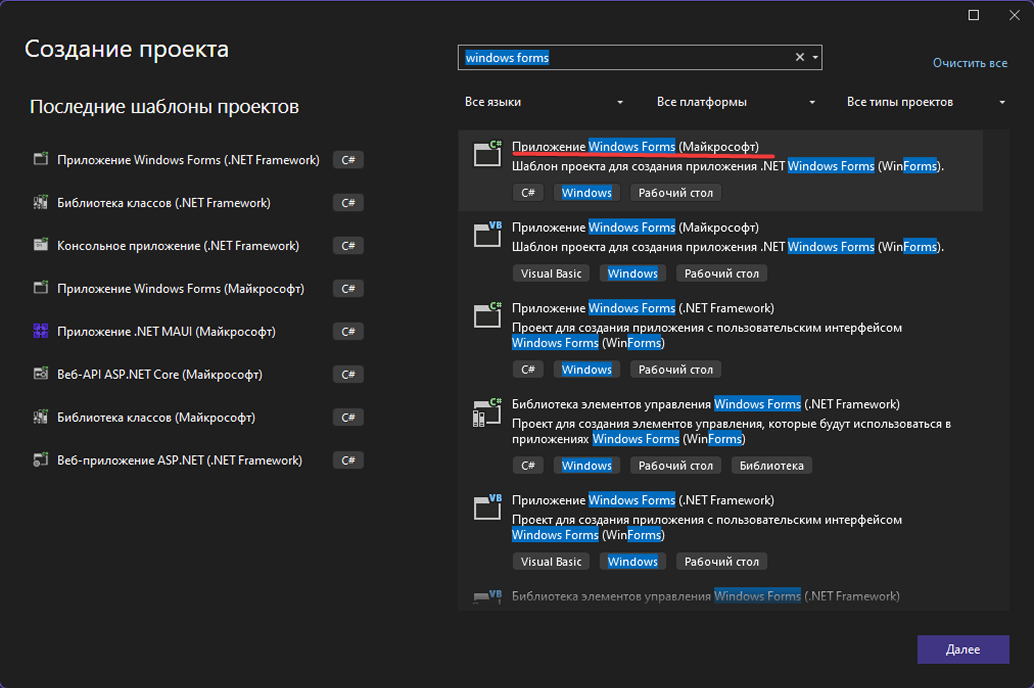
\includegraphics[width=0.6\textwidth]{fig/image-3.jpg}
	\caption{Обозначения разделов}
	\label{fig:Обозначения разделов}
\end{figure}

\begin{itemize}
	\item Указываете название формы (содержащее номер лабораторной работы).
	\item Выбираете последнюю версию платформы из доступных (в примере \texttt{.NET 8.0}) (Рисунок~\ref{fig:Настройки проекта}).
\end{itemize}

\begin{figure}[H]
	\centering
	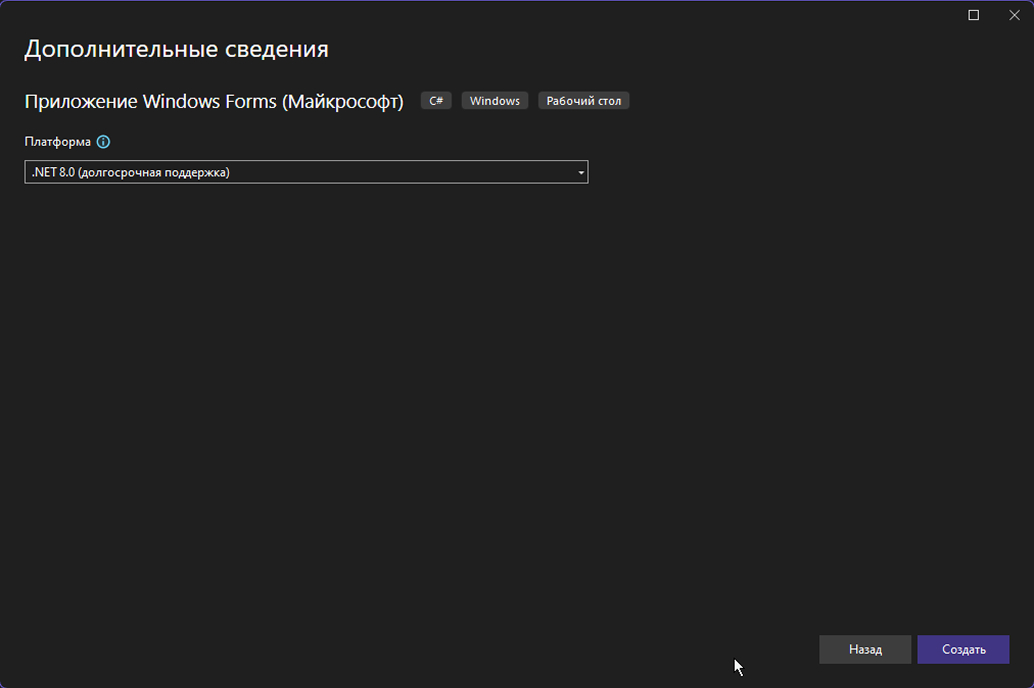
\includegraphics[width=0.6\textwidth]{fig/image-2.jpg}
	\caption{Настройки проекта}
	\label{fig:Настройки проекта}
\end{figure}

Перед вами откроется проект с формой по умолчанию.
Слева будет <<Панель элементов>> (если ее нет, перейти в <<Вид>> \iicon{} <<Панель элементов>> / \texttt{Ctrl + Alt + X}) (Рисунок~\ref{fig:Окно проекта}).

\begin{figure}[H]
	\centering
	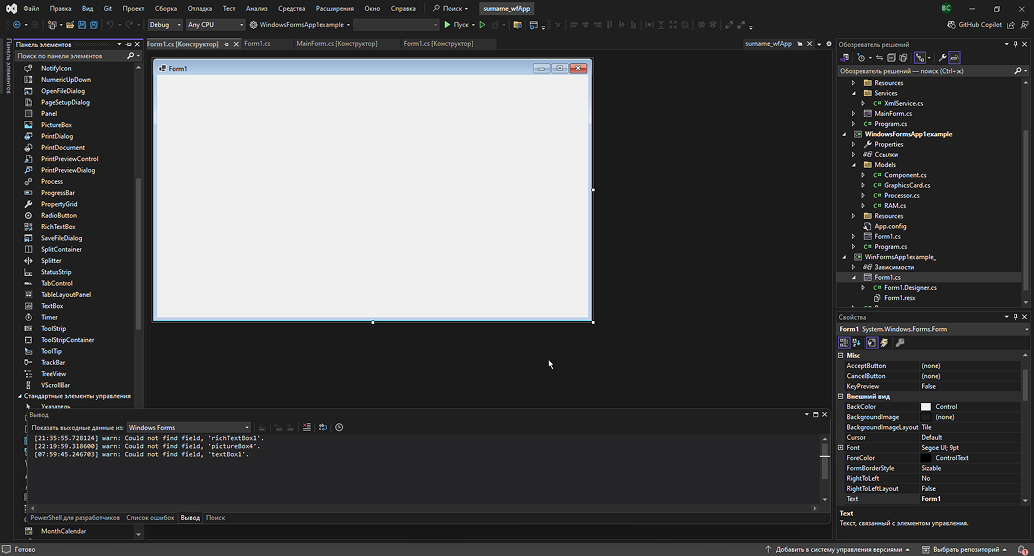
\includegraphics[width=0.8\textwidth]{fig/image-1.jpg}
	\caption{Окно проекта}
	\label{fig:Окно проекта}
\end{figure}

\newpage

\section{Основные элементы Windows Forms}

Панель элементов содержит множество элементов для работы с формами.
Можно выделить наиболее часто используемые:
\begin{itemize}
	\item \textbf{\texttt{Form:}}
	      Основное окно приложения. Служит контейнером для других элементов управления, предоставляет базовую функциональность для создания пользовательского интерфейса (размещение, масштабирование, обработка событий формы).
	\item \textbf{\texttt{Button:}}
	      Кнопка, по нажатию на которую происходит выполнение заданного кода. Используется для инициирования действий (например, отправка данных, переход на другую форму).
	\item \textbf{\texttt{Label:}}
	      Элемент для отображения текста. Предназначен для вывода информационных сообщений, описания других элементов и инструкций. Не поддерживает ввод данных.
	\item \textbf{\texttt{TextBox:}}
	      Поле для ввода и отображения однострочного текста. Используется для сбора пользовательского ввода, поиска, ввода паролей (с установкой \texttt{PasswordChar}) и т.д.
	\item \textbf{\texttt{RichTextBox:}}
	      Расширенная версия \texttt{TextBox}, позволяющая форматировать текст (изменять шрифты, цвета, стили). Полезна для редактирования многострочного форматированного текста.
	\item \textbf{\texttt{CheckBox:}}
	      Флажок, позволяющий выбирать или снимать выбор (логическое значение \texttt{true} или \texttt{false}). Применяется в формах для подтверждения, включения настроек и т.п.
	\item \textbf{\texttt{ListBox:}}
	      Список, позволяющий отображать набор элементов, из которых пользователь может выбрать один или несколько. Простой способ представления данных в виде списка.
	\item \textbf{\texttt{ComboBox:}}
	      Комбинированный элемент, который сочетает в себе поле для ввода и выпадающий список. Удобен для выбора одного значения из набора, позволяя пользователю как выбрать из списка, так и ввести значение вручную.
	\item \textbf{\texttt{ListView:}}
	      Многофункциональный список с поддержкой различных видов отображения (иконки, подробности, плитка). Позволяет отображать элементы с подэлементами, а также использовать возможности сортировки и фильтрации (но редактирование ограничено).
	\item \textbf{\texttt{DataGridView:}}
	      Табличное представление данных с поддержкой привязки данных, сортировки, фильтрации и встроенного редактирования ячеек.
	\item \textbf{\texttt{PictureBox:}}
	      Элемент для отображения изображений. Поддерживает различные форматы, позволяет масштабировать или изменять размер изображения в соответствии с настройками.
	\item \textbf{\texttt{Panel:}}
	      Контейнер для других элементов управления, позволяющий группировать связанные элементы и управлять их компоновкой. Может использоваться для создания сложных макетов или динамического отображения или скрытия групп элементов.
	\item \textbf{\texttt{GroupBox:}}
	      Контейнер с рамкой и заголовком, предназначенный для группировки элементов управления, которые логически связаны между собой. Улучшает визуальную организацию интерфейса.
	\item \textbf{\texttt{MenuStrip:}}
	      Панель меню, располагаемая обычно в верхней части формы. Позволяет создавать выпадающие меню (например, Файл, Правка, Вид и т.д.) для доступа к командам приложения.
	\item \textbf{\texttt{ToolStrip:}}
	      Панель инструментов, содержащая кнопки, текстовые поля, комбобоксы и другие элементы, предназначенные для быстрого доступа к функциям приложения.
	\item \textbf{\texttt{StatusStrip:}}
	      Элемент, располагаемый в нижней части формы, для отображения статусной информации (например, индикаторы, сообщения, время работы).
	\item \textbf{\texttt{TabControl:}}
	      Элемент, позволяющий создавать вкладки для организации контента в пределах одного окна. Удобен для разделения функциональности на логически связанные секции.
\end{itemize}

\newpage

\section{Шаг 2. Создание формы \ \texorpdfstring{{\small{\iicon{}}}}{}}
Для примера будет разработана форма, содержащая следующие элементы:
\begin{enumerate}
	\item \texttt{DataGridView} -- для добавления элементов и отображения их в табличном виде.
	\item \texttt{Button} -- для добавления элементов, удаления и поиска.
	\item \texttt{TextBox} -- для ввода необходимых данных при добавлении элемента или поиске.
	\item \texttt{PictureBox} -- для добавления изображения.
	\item \texttt{Panel} -- для группировки элементов, создания <<вкладок>>.
	\item \texttt{Label} -- для подписи элементов.
\end{enumerate}

Необходимо разместить соответствующие элементы на форме (пока что схематично). Пример формы изображен на рисунке~\ref{fig:Пример оформления формы}.

\begin{figure}[H]
	\centering
	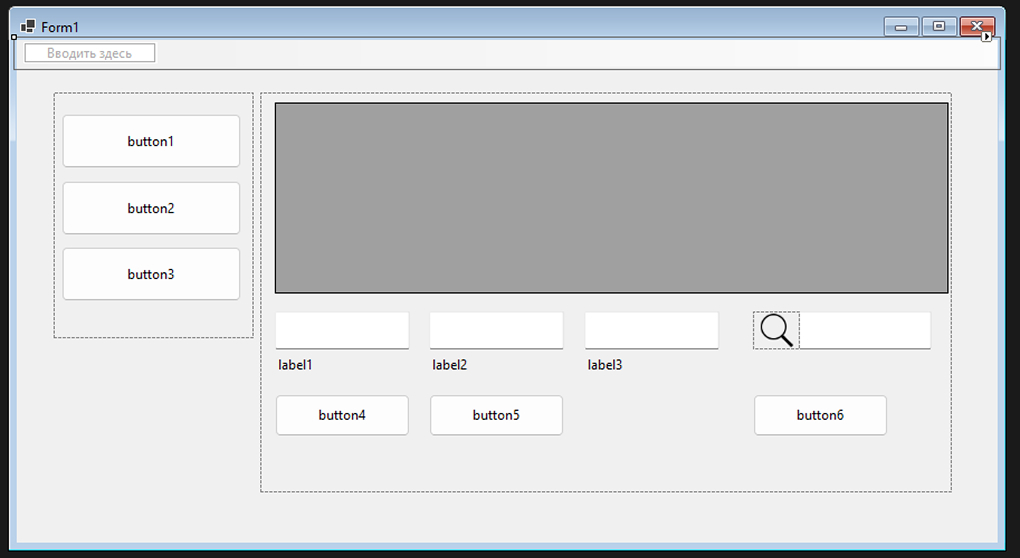
\includegraphics[width=0.6\textwidth]{fig/image.jpg}
	\caption{Пример оформления формы}
	\label{fig:Пример оформления формы}
\end{figure}

Возвращаясь к настройке внешнего вида формы, необходимо рассмотреть свойства элементов формы. В правом нижнем углу в проекте можно увидеть окно свойств элемента. Рассмотрим основные свойства, настройка которых потребуется для создания интуитивного и понятного интерфейса, а также изменения внешнего вида элементов.
В верхней части панели есть кнопки для сортировки и перехода по разделам (свойства, эффекты). Для того, чтобы быстрее найти нужное свойство, можно выбрать сортировку <<по категориям>>.
Для того чтобы изменить название элемента в коде (при обращении к нему, вызове метода), используется свойство (\texttt{Name}). Его можно найти в разделе <<Design>> (<<Разработка>>) (Рисунок~\ref{fig:101}).

\begin{figure}[H]
	\centering
	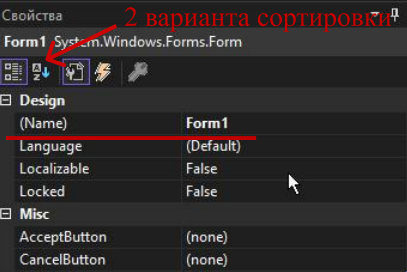
\includegraphics[width=0.6\textwidth]{fig/100.png}
	\caption{Свойство Name}
	\label{fig:101}
\end{figure}

\footnotetext{Подробно про свойства можно почитать по ссылке: \url{https://metanit.com/sharp/windowsforms/2.2.php}}

Для того чтобы изменить текст, отображаемый на элементе, необходимо указать новое название в свойстве <<\texttt{Text}>> в разделе <<Внешний вид>> (Рисунок~\ref{fig:Свойство text}).

\begin{figure}[H]
	\centering
	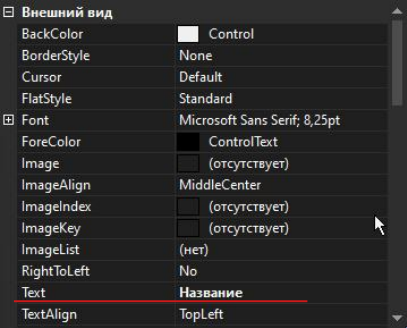
\includegraphics[width=0.6\textwidth]{fig/101.png}
	\caption{Свойство \texttt{text}}
	\label{fig:Свойство text}
\end{figure}

Также можно использовать свойство \texttt{PlaceholderText}, чтобы изменить текст, отображаемый на элементе. Свойство находится в разделе <<Misc>> (Рисунок~\ref{fig:Свойство Placeholder}). Данное свойство доступно при создании проекта Майкрософт.

\begin{figure}[H]
	\centering
	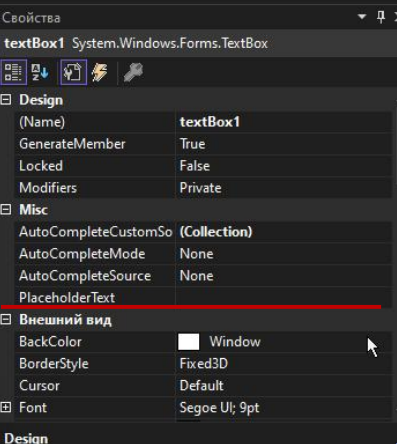
\includegraphics[width=0.6\textwidth]{fig/102.png}
	\caption{Свойство \texttt{Placeholder}}
	\label{fig:Свойство Placeholder}
\end{figure}

Также необходимо настроить внешний вид элемента \texttt{TextBox}. Для того чтобы изменить высоту \texttt{TextBox}, необходимо изменить значение параметра \texttt{Multiline} на \texttt{True} (Рисунок~\ref{fig:Свойство Multiline}).

\begin{figure}[H]
	\centering
	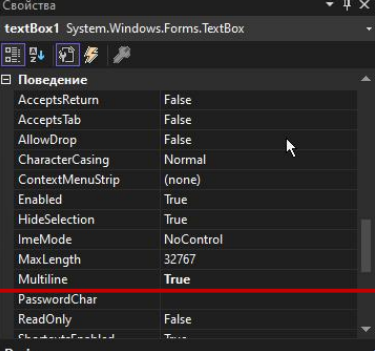
\includegraphics[width=0.6\textwidth]{fig/103.png}
	\caption{Свойство \texttt{Multiline}}
	\label{fig:Свойство Multiline}
\end{figure}

Для изменения фонового цвета используется свойство \texttt{BackColor}, а для изменения цвета текста -- \texttt{ForeColor} (Рисунок~\ref{fig:Свойства для изменения цвета}).


\begin{figure}[H]
	\centering
	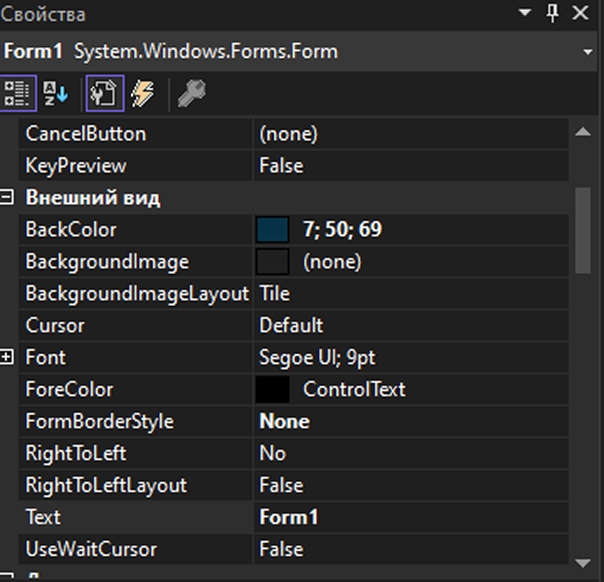
\includegraphics[width=0.6\textwidth]{fig/image 58.jpg}
	\caption{Свойства для изменения цвета}
	\label{fig:Свойства для изменения цвета}
\end{figure}

Применив необходимые изменения, получим форму, изображенную на рисунке~\ref{fig:Стилизация интерфейса на ваше умотрение smileface}.

\begin{figure}[H]
	\centering
	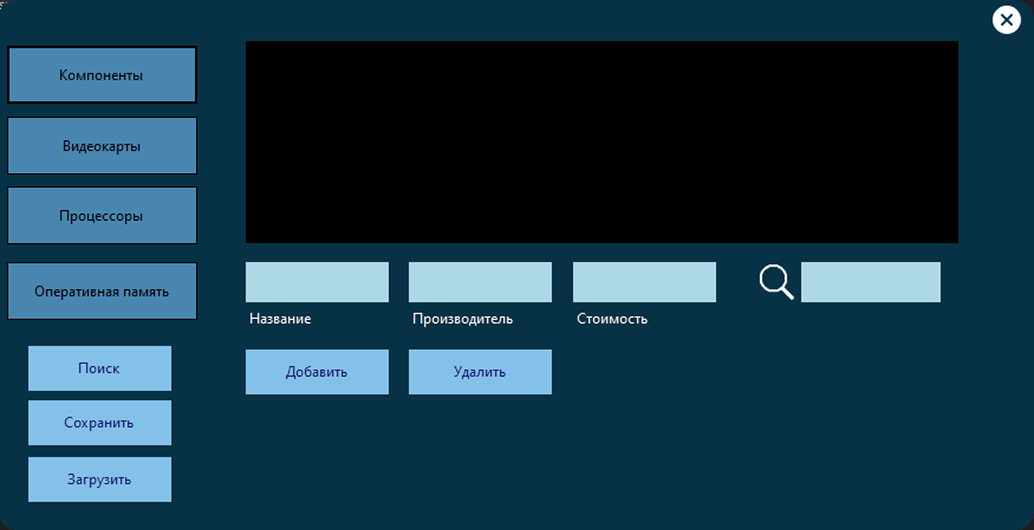
\includegraphics[width=0.8\textwidth]{fig/image 37.jpg}
	\caption{Пример стилизованной формы\protect\footnotemark}
	\label{fig:Стилизация интерфейса на ваше умотрение smileface}
\end{figure}
\footnotetext{Стилизация интерфейса на ваше усмотрение {\scriptsize{\iicon{}}}}

Важно учесть расположение форм, которые в данном случае находятся друг над другом. Расположение панелей на форме указано на рисунке~\ref{fig:Структура формы}.

\begin{figure}[H]
	\centering
	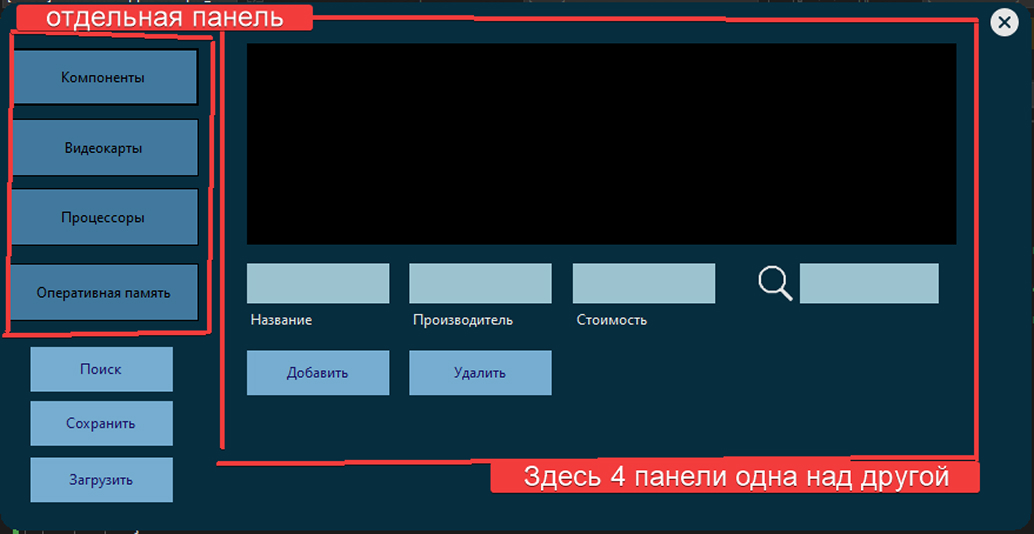
\includegraphics[width=0.6\textwidth]{fig/image 38.jpg}
	\caption{Структура формы}
	\label{fig:Структура формы}
\end{figure}

Также для более детального рассмотрения и управления положением элементов на форме можно воспользоваться окном <<Структура документа>> (Вид \iicon{} Другие окна \iicon{} Структура документа), для этого нужно открыть файл с самой формой (\texttt{Form.cs}). Структура документа изображена на рисунке~\ref{fig:Структура формы2}.

\begin{figure}[H]
	\centering
	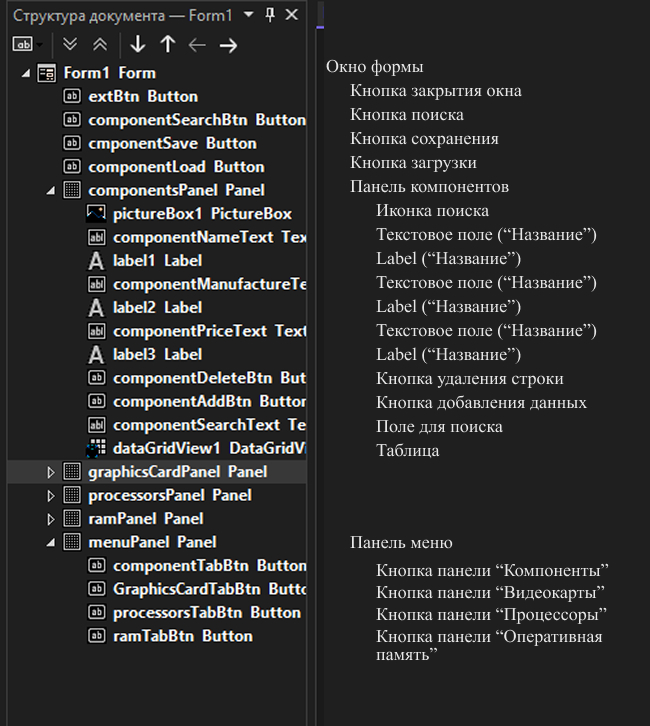
\includegraphics[width=0.6\textwidth]{fig/Group 98.jpg}
	\caption{Структура формы}
	\label{fig:Структура формы2}
\end{figure}

\newpage

\section{Шаг 3. Добавление классов \ \texorpdfstring{{\small{\iicon{}}}}{}}

Далее необходимо в Решении создать папку и добавить туда классы из лабораторной 1 (Рисунок~\ref{fig:Создание классов для работы с данными в форме}).

\begin{figure}[H]
	\centering
	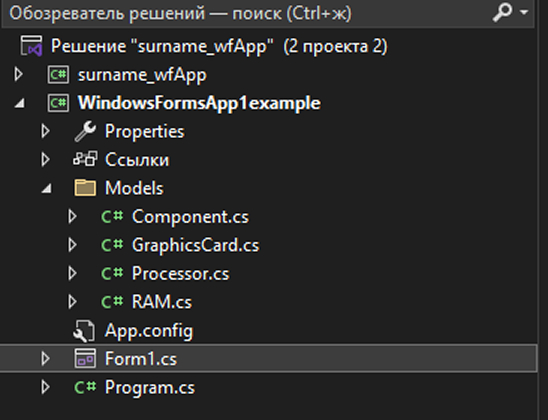
\includegraphics[width=0.6\textwidth]{fig/image 5.jpg}
	\caption{Создание классов для работы с данными в форме}
	\label{fig:Создание классов для работы с данными в форме}
\end{figure}

В каждом классе необходимо наличие 3 свойств, конструктора без параметров (нужен для сериализации) и конструктора с параметрами (Листинг~\ref{lst:OrderCs}).

\begin{code}
	\inputminted[firstline = 9, fontsize=\fontsize{9pt}{10pt}]{csharp}{../2lab/surname_wfApp/Models/Component.cs}
	\caption{Пример структуры \colorGIT{\href{https://github.com/WebMasterIT/Csharp_Labs/blob/c79e983c4cab3c416e44b6d5f9854b292fdeae26/2lab/surname_wfApp/Models/Component.cs}{класса}}}
	\label{lst:OrderCs}
\end{code}

\newpage

\section{Шаг 4. Реализация добавления данных в таблицу \ \texorpdfstring{{\small{\iicon{}}}}{}}

После добавления классов необходимо настроить обработчики событий.
В \texttt{WinForms} у элементов управления (кнопок, чекбоксов, текстовых полей и т. д.) есть события (\texttt{events}), которые вызываются при определенных действиях пользователя.
Например, клик по кнопке является одним из событий и при настройке появляется в окне свойств (Рисунок~\ref{fig:Добавление событий}).

\begin{figure}[H]
	\centering
	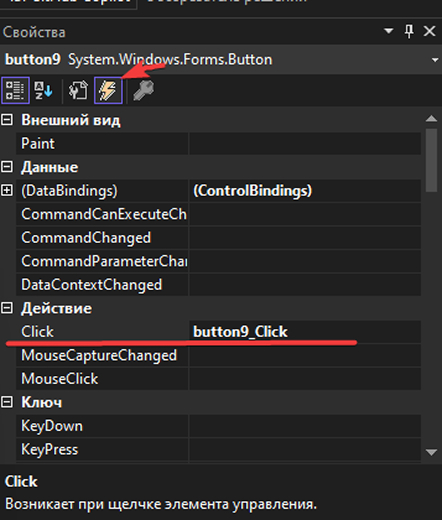
\includegraphics[width=0.6\textwidth]{fig/image 31.jpg}
	\caption{Добавление событий}
	\label{fig:Добавление событий}
\end{figure}

Если настраиваемое событие не отрабатывает, необходимо проверить панель свойств на наличие события в данном разделе.

Далее необходимо добавить событие нажатия на кнопку добавления данных в таблицу. Пример метода для добавления данных в форму представлен в листинге~\ref{lst: Методы добавления данных в форму}.

\begin{code}
	\inputminted[firstline = 165, lastline=200]{csharp}{../2lab/WinFormsApp1example_/Form1.cs}
	\caption{\colorGIT{\href{https://github.com/WebMasterIT/Csharp_Labs/blob/c79e983c4cab3c416e44b6d5f9854b292fdeae26/2lab/WinFormsApp1example_/Form1.cs\#L165-L200}{Метод}} добавления данных в форму}
	\label{lst: Методы добавления данных в форму}
\end{code}

Также необходимо после добавления данных обновить данные в таблице (\texttt{DataGridView}) (Листинг~\ref{lst:Метод обновления Datagridview}).

\begin{code}
	\inputminted[firstline = 234, lastline=277]{csharp}{../2lab/WinFormsApp1example_/Form1.cs}
	\caption{\colorGIT{\href{https://github.com/WebMasterIT/Csharp_Labs/blob/c79e983c4cab3c416e44b6d5f9854b292fdeae26/2lab/WinFormsApp1example_/Form1.cs\#L234-L277}{Метод}} обновления \texttt{DataGridView}}
	\label{lst:Метод обновления Datagridview}
\end{code}


Можно также добавить событие удаления элемента (строки) из таблицы (Листинг~\ref{lst:Метод удаления строки из Datagridview}).

\begin{code}
	\inputminted[firstline = 346, lastline=363]{csharp}{../2lab/WinFormsApp1example_/Form1.cs}
	\caption{\colorGIT{\href{https://github.com/WebMasterIT/Csharp_Labs/blob/c79e983c4cab3c416e44b6d5f9854b292fdeae26/2lab/WinFormsApp1example_/Form1.cs\#L346-L363}{Метод}} удаления строки из \texttt{DataGridView}}
	\label{lst:Метод удаления строки из Datagridview}
\end{code}

Для добавления данных в заранее созданные поля, необходимо связать название поля со свойствами создаваемого объекта (Листинг~\ref{lst:Добавления данных в столбцы DataGridView без автогенерации}).

\begin{code}
	\inputminted[firstline=146, lastline=163]{csharp}{../2lab/WinFormsApp1example_/Form1.cs}
	\caption{\colorGIT{\href{https://github.com/WebMasterIT/Csharp_Labs/blob/c79e983c4cab3c416e44b6d5f9854b292fdeae26/2lab/WinFormsApp1example_/Form1.cs\#L146-L163}{Добавление}} данных в столбцы \texttt{DataGridView} без автогенерации}
	\label{lst:Добавления данных в столбцы DataGridView без автогенерации}
\end{code}

Важно при работе с панелями динамически скрывать и делать их видимыми при выборе соответствующей вкладки. Для этого необходимо создать метод, который будет менять свойство \texttt{Visible} у соответствующей панели при нажатии на кнопку (Листинг~\ref{lst:Метод скрытия панелей}).

\begin{code}
	\inputminted[firstline = 100, lastline=131]{csharp}{../2lab/WinFormsApp1example_/Form1.cs}
	\caption{\colorGIT{\href{https://github.com/WebMasterIT/Csharp_Labs/blob/c79e983c4cab3c416e44b6d5f9854b292fdeae26/2lab/WinFormsApp1example_/Form1.cs\#L100-L131}{Метод}} скрытия панелей}
	\label{lst:Метод скрытия панелей}
\end{code}

\newpage

\section{Шаг 5. Реализация фильтрации (поиска) данных \ \texorpdfstring{{\small{\iicon{}}}}{}}
Для поиска нужных данных в таблице используется поиск по подстроке в каждом столбце (листинг~\ref{lst:Метод фильтрации (поиска) данных в таблице}).

\begin{code}
	\inputminted[firstline = 280, lastline=341, fontsize={\fontsize{8}{8.4}}]{csharp}{../2lab/WinFormsApp1example_/Form1.cs}
	\caption{\colorGIT{\href{https://github.com/WebMasterIT/Csharp_Labs/blob/c79e983c4cab3c416e44b6d5f9854b292fdeae26/2lab/WinFormsApp1example_/Form1.cs\#L280-L341}{Метод}} фильтрации (поиска) данных в таблице}
	\label{lst:Метод фильтрации (поиска) данных в таблице}
\end{code}

\newpage

\section{Шаг 6. Сериализация, десериализация классов. Сохранение в XML \ \texorpdfstring{{\small{\iicon{}}}}{}}

\textbf{Сериализация} -- это процесс преобразования объекта в поток байтов для его сохранения в файле, передаче по сети или хранении в базе данных. Впоследствии этот объект можно восстановить (десериализовать).

Типы сериализации в \texttt{C\#}

В \texttt{C\#} есть несколько типов сериализации:
\begin{itemize}
	\item \texttt{Binary}
	\item \texttt{XML}
	\item \texttt{JSON}
	\item \texttt{CSV}\footnote{Это простой текстовый формат для хранения табличных данных, где каждая строка файла представляет одну строку таблицы. Значения в каждой строке разделяются определенным символом, чаще всего запятой.}
	\item \ldots
\end{itemize}

В данном случае будет рассмотрена \texttt{XML}-сериализация. В \texttt{C\#} для работы с \texttt{XML} используется класс \texttt{XmlSerializer} из пространства имен \texttt{System.Xml.Serialization}.

Пример метода сериализации с использованием \texttt{List} приведен в листинге~\ref{lst:Пример метода сериализации классов}.

\begin{code}
	\inputminted[firstline = 531, lastline=598, fontsize=\fontsize{8pt}{10pt}]{csharp}{../2lab/WinFormsApp1example_/Form1.cs}
	\captionof{listing}{\colorGIT{\href{https://github.com/WebMasterIT/Csharp_Labs/blob/c79e983c4cab3c416e44b6d5f9854b292fdeae26/2lab/WinFormsApp1example_/Form1.cs\#L531-L598}{Пример}} сериализации данных с помощью \texttt{DataTable}}
	\label{lst:Пример метода сериализации классов}
\end{code}


\noindent Объяснение ключевых моментов:
\begin{itemize}
	\item \textbf{\texttt{SaveFileDialog:}}
	      Используется для взаимодействия с пользователем, чтобы выбрать место и имя файла. \texttt{Filter} ограничивает выбор \texttt{XML}-файлами, но позволяет выбрать <<все файлы>> (\texttt{*.*}).
	\item \textbf{\texttt{XmlSerializer:}}
	      Инструмент для преобразования объектов \texttt{C\#} (в данном случае списков \texttt{List\-<T>}) в \texttt{XML}-формат и обратно. Он требует, чтобы классы (\texttt{Component}, \texttt{GraphicsCard}, \texttt{Processor}) имели публичные свойства и пустой конструктор.
	\item \textbf{\texttt{using (TextWriter ...):}}
	      Обеспечивает корректное закрытие файла после записи, даже если произойдёт ошибка.
	\item \textbf{Проверка на пустой список:}
	      Перед сериализацией проверяется \texttt{Count}, чтобы не создавать пустой \texttt{XML}-файл.
	\item \textbf{Условные ветви (\texttt{if-else}):}
	      Код определяет, какой список сериализовать, основываясь на активном \texttt{DataGridView}. Это позволяет сохранять данные только для текущей вкладки.
\end{itemize}

Также можно использовать сериализацию данных с помощью \texttt{DataTable}, не используя списки \texttt{List} (Листинг~\ref{fig:Серилилация данных через DataTable}).

\begin{code}
	\begin{minted}{csharp}
private void SaveDataGridView(DataGridView dgv)
{
    // Создаем и настраиваем диалог сохранения файла
    using (SaveFileDialog saveFileDialog = new SaveFileDialog { Filter = "XML файлы|*.xml", Title = "Сохранить данные" })
    {
        // Проверяем, нажал ли пользователь кнопку "Сохранить"
        if (saveFileDialog.ShowDialog() == DialogResult.OK)
        {
            // Создаем DataTable с именем "MyTable"
            DataTable dt = new DataTable("MyTable");

            // Добавляем в DataTable колонки из DataGridView
            foreach (DataGridViewColumn column in dgv.Columns)
            {
                dt.Columns.Add(column.Name);
            }

            // Перебираем все строки DataGridView
            foreach (DataGridViewRow row in dgv.Rows)
            {
                // Пропускаем строку, если она новая (пустая)
                if (!row.IsNewRow)
                {
                    // Создаем новую строку для DataTable
                    DataRow dr = dt.NewRow();

                    // Заполняем строку данными из ячеек DataGridView
                    for (int i = 0; i < dgv.Columns.Count; i++)
                    {
                        dr[i] = row.Cells[i].Value ?? DBNull.Value; // Если значение null, заменяем его на DBNull.Value
                    }

                    // Добавляем заполненную строку в DataTable
                    dt.Rows.Add(dr);
                }
            }

            // Сохраняем DataTable в XML-файл с указанием схемы
            dt.WriteXml(saveFileDialog.FileName, XmlWriteMode.WriteSchema);

            // Выводим сообщение об успешном сохранении данных
            MessageBox.Show("Данные сохранены!", "Успех", MessageBoxButtons.OK, MessageBoxIcon.Information);
        }
    }
}
	\end{minted}
	\captionof{listing}{Пример сериализации данных с помощью \texttt{DataTable}}
	\label{fig:Серилилация данных через DataTable}
\end{code}

\begin{code}
	\inputminted[firstline = 467, lastline=521]{csharp}{../2lab/WinFormsApp1example_/Form1.cs}
	\captionof{listing}{Пример \colorGIT{\href{https://github.com/WebMasterIT/Csharp_Labs/blob/c79e983c4cab3c416e44b6d5f9854b292fdeae26/2lab/WinFormsApp1example_/Form1.cs\#L467-L521}{метода}} десериализации\protect\footnotemark}
\end{code}

\footnotetext{Десериализация -- это процесс обратного преобразования, то есть восстановления объекта из сохраненного состояния.}

\noindent Разбор метода десериализации.


\begin{code}
	\inputminted[firstline = 467, lastline=468]{csharp}{../2lab/WinFormsApp1example_/Form1.cs}
	\captionof{listing}{\colorGIT{\href{https://github.com/WebMasterIT/Csharp_Labs/blob/c79e983c4cab3c416e44b6d5f9854b292fdeae26/2lab/WinFormsApp1example_/Form1.cs\#L467-L468}{Метод}} десериализации с параметром}
	\label{lst:method dis}
\end{code}

Метод принимает параметр \texttt{dgv} типа \texttt{DataGridView}, чтобы знать, в какой \texttt{DataGridView} нужно загрузить данные (например, \texttt{dataGridView4} для процессоров, \texttt{dataGridView1} для компонентов или \texttt{dataGridView2} для видеокарт). Такой подход делает метод универсальным -- он может работать с любым \texttt{DataGridView}, а не с конкретным. Это удобно, если у вас несколько таблиц (\texttt{dataGridView1}, \texttt{dataGridView2}, \texttt{dataGridView4}), и вы хотите переиспользовать код (Листинг~\ref{lst:method dis}).

\begin{code}
	\inputminted[firstline = 470, lastline=472]{csharp}{../2lab/WinFormsApp1example_/Form1.cs}
	\captionof{listing}{\colorGIT{\href{https://github.com/WebMasterIT/Csharp_Labs/blob/c79e983c4cab3c416e44b6d5f9854b292fdeae26/2lab/WinFormsApp1example_/Form1.cs\#L470-L472}{Объект}} \texttt{OpenFileDialog}}
	\label{lst:OpenFileDialog}
\end{code}

Создаётся объект \texttt{OpenFileDialog} для выбора файла пользователем. Свойство \texttt{Filter} задаёт фильтр файлов, чтобы в диалоге отображались только \texttt{XML}-файлы по умолчанию, но с возможностью выбрать <<все файлы>>. Фильтр упрощает пользователю выбор нужного файла, показывая только файлы с расширением \texttt{.xml}.

Формат фильтра \texttt{\detokenize{"XML Files (*.xml)|*.xml|All Files (*.*)|*.*"}} -- это стандартный синтаксис для \texttt{OpenFileDialog}. Первая часть (\texttt{\detokenize{XML Files (*.xml)}}) -- это описание, вторая (\texttt{\detokenize{*.xml}}) -- маска файлов. Аналогично для \texttt{\detokenize{"All Files"}} (Листинг~\ref{lst:OpenFileDialog}).

\begin{code}
	\inputminted[firstline = 474, lastline=482]{csharp}{../2lab/WinFormsApp1example_/Form1.cs}
	\captionof{listing}{Выбор файла и \colorGIT{\href{https://github.com/WebMasterIT/Csharp_Labs/blob/c79e983c4cab3c416e44b6d5f9854b292fdeae26/2lab/WinFormsApp1example_/Form1.cs\#L474-L482}{проверка}} на корректную таблицу}
	\label{lst:table}
\end{code}

Метод \texttt{ShowDialog()} (Листинг~\ref{lst:table}) открывает диалоговое окно выбора файла. Если пользователь выбрал файл и нажал <<Открыть>>, возвращается \texttt{DialogResult.OK}. Если пользователь нажал <<Отмена>>, метод завершится, ничего не делая.

Свойство \texttt{FileName} возвращает полный путь к выбранному файлу (например, \texttt{C:\textbackslash{}data.xml}). Этот путь нужен для чтения данных из файла. Без пути не получится открыть файл для десериализации.

\begin{code}
	\begin{minted}{csharp}
        if (dgv == null)
        {
            MessageBox.Show("Передан некорректный DataGridView для загрузки данных.");
            return;
        }
    \end{minted}
\end{code}


Проверяется, что переданный \texttt{DataGridView} (\texttt{dgv}) не равен \texttt{null}. Если \texttt{dgv} равен \texttt{null}, дальнейшая работа с ним вызовет исключение \texttt{NullReferenceException}. Эта проверка защищает от таких ошибок.

\begin{code}
	\inputminted[firstline = 485, lastline=493]{csharp}{../2lab/WinFormsApp1example_/Form1.cs}
	\captionof{listing}{\colorGIT{\href{https://github.com/WebMasterIT/Csharp_Labs/blob/c79e983c4cab3c416e44b6d5f9854b292fdeae26/2lab/WinFormsApp1example_/Form1.cs\#L485-L493}{Сериализация}} \texttt{XML}}
	\label{lst:ser XML}
\end{code}

Далее рассмотрим объект \texttt{XmlSerializer}, позволяющий сохранять данные из таблицы в формате \texttt{XML} (Листинг~\ref{lst:ser XML}).

Если переданный \texttt{DataGridView} -- это \texttt{dataGridView1} (для компонентов), данные загружаются в \texttt{componentList}. Создаётся объект \texttt{XmlSerializer} для типа \texttt{List<Component>}. \texttt{XmlSerializer} знает, как преобразовать \texttt{XML} в список объектов \texttt{Component}; это указывает, что ожидается \texttt{XML}-файл, содержащий список объектов \texttt{Component}.

\texttt{StreamReader} открывает файл по пути \texttt{filePath} для чтения текста.
Конструкция \texttt{using} гарантирует, что поток (\texttt{StreamReader}) будет закрыт после использования, даже если произойдёт исключение.

Метод \texttt{Deserialize} читает \texttt{XML} из потока и преобразует его в объект типа \texttt{List<Component>}.
Приведение \texttt{(List<Component>)} необходимо, так как \texttt{Deserialize} возвращает объект типа \texttt{object}. Сбрасывается фильтр, чтобы после загрузки отображался полный список компонентов, а не отфильтрованный. Этот блок загружает данные из \texttt{XML}-файла в список \texttt{componentList}, который привязан к \texttt{dataGridView1}. Сброс фильтра (\texttt{filteredComponentList = null}) гарантирует, что пользователь увидит все загруженные данные.

Почему так: Использование \texttt{XmlSerializer} -- это стандартный способ десериализации \texttt{XML} в \texttt{.NET}. Проверка \texttt{dgv == dataGridView1} позволяет методу работать с разными \texttt{DataGridView} и списками.
Также важно связать события кнопок сохранения и загрузки с соответствующими таблицами (Листинг~\ref{lst:Tag}).

\begin{code}
	\inputminted[firstline = 146, lastline = 163]{csharp}{../2lab/WinFormsApp1example_/Form1.cs}
	\caption{Связь событий и кнопок с помощью \colorGIT{\href{https://github.com/WebMasterIT/Csharp_Labs/blob/c79e983c4cab3c416e44b6d5f9854b292fdeae26/2lab/WinFormsApp1example_/Form1.cs\#L146-L163}{\texttt{Tag}}}}
	\label{lst:Tag}
\end{code}

\newpage

\section{Дополнительная информация~\texorpdfstring{\iicon{}}{}}

\begin{enumerate}
	\item Обязательно ли указывать атрибут \texttt{Serializable}? \\
	      Нет, атрибут \texttt{[Serializable]} не нужен, если используется \texttt{DataSet} / \texttt{DataTable} + \texttt{XML} для сохранения данных.

	\item Почему \texttt{Serializable} не важен? \\
	      Атрибут \texttt{[Serializable]} требуется, если объекты сохраняются с помощью бинарной или \texttt{JSON}-сериализации (например, \texttt{BinaryFormatter} или \texttt{JsonSerializer}).

	      \textcolor{CtpRed}{НО} при использовании \texttt{DataSet.WriteXml(filePath)} не нужно указывать атрибут, так как:
	      \begin{itemize}
		      \item[\iicon{󰄬}] \texttt{DataSet.WriteXml(filePath)} сохраняет данные в \texttt{XML} без необходимости сериализации класса.
		      \item[\iicon{󰄬}] Работает с таблицами (\texttt{DataTable}), а не с объектами конкретного \texttt{List}.
	      \end{itemize}

	      Когда \texttt{[Serializable]} был бы нужен:
	      \begin{itemize}
		      \item Если объекты \texttt{List} сохраняются в файл (например, \texttt{JSON}, \texttt{Binary}, \texttt{SOAP}).
		      \item Если используется \texttt{BinaryFormatter} или \texttt{JsonConvert.Serialize\-Object(graphics\-CardList)}
	      \end{itemize}
\end{enumerate}

Если необходимо добавлять данные в уже созданные ячейки \texttt{DataGridView}, а не создавать новые строки, необходимо обновлять значения ячеек в существующих строках. Это можно сделать несколькими способами:

\begin{enumerate}
	\item Обращение к ячейкам по индексу строки и столбца.

	      В случае, если в \texttt{DataGridView} уже присутствуют строки, можно обновлять данные так:

	      \begin{minted}{csharp}
                // Обновление данных в первой строке (индекс 0)
                dataGridView1.Rows[0].Cells[0].Value = "Новое значение";
                dataGridView1.Rows[0].Cells[1].Value = 123;
          \end{minted}

	\item Работа с \texttt{DataTable} (если \texttt{DataGridView} привязан к нему).

	      Если \texttt{DataGridView} использует \texttt{DataTable} как источник данных:

	      \begin{minted}{csharp}
                // Получаем доступ к DataTable
                DataTable dt = (DataTable)dataGridView1.DataSource; // Изменяем данные в нужной строке и столбце
                dt.Rows[0]["НазваниеСтолбца"] = "Новое значение";
          \end{minted}

	      После этого \texttt{DataGridView} обновится автоматически.

	\item Обновление данных через \texttt{BindingList<T>}.

	      Если \texttt{DataGridView} привязан к \texttt{BindingList<T>}, можно менять объект в списке:

	      \begin{minted}{csharp}
                // Предположим, у нас есть BindingList<MyObject> bindingList;
                // bindingList[0].SomeProperty = "Новое значение";
                dataGridView1.Refresh(); // Принудительно обновляем DataGridView
          \end{minted}
\end{enumerate}

\noindent \textcolor{CtpRed}{Важно:}
\begin{itemize}
	\item Убедитесь, что строки уже существуют перед обновлением (\texttt{dataGridView1.Rows.Count}).
	\item Если \texttt{DataGridView} связан с \texttt{DataTable} или \texttt{BindingList<T>}, изменения надо делать в источнике данных.
\end{itemize}

\newpage

\section{Стилизация интерфейса~~\texorpdfstring{\iicon{}}{}}

% \begin{figure}[H]
% 	\centering
% 	\includegraphics[width=0.8\textwidth]{img/page_40_image_1.png} % Placeholder
% 	\caption{Свойство FormBorderStyle}
% 	\label{fig:6.9}
% \end{figure}

После этого возможность перемещать форму с помощью мыши будет отключена. Чтобы вернуть возможность перемещения формы, необходимо добавить флаги для реализации перемещения формы, функции для перемещения формы и обработчики событий нажатия мыши. Также можно стилизовать форму, закруглив края с помощью функции \texttt{CreateRoundRectRgn}.

Флаги для реализации перемещения формы и функции для перемещения формы, а также функции для скругления краев формы представлены в листинге \ref{list:6.10}.

\begin{code}
	\inputminted[firstline = 22, lastline=45]{csharp}{../2lab/WinFormsApp1example_/Form1.cs}
	\caption{\colorGIT{\href{https://github.com/WebMasterIT/Csharp_Labs/blob/c79e983c4cab3c416e44b6d5f9854b292fdeae26/2lab/WinFormsApp1example_/Form1.cs\#L22-L45}{Функции}} реализации перемещения формы}
	\label{list:6.10}
\end{code}

Обработчики нажатия мыши приведены в листинге \ref{list:6.11}.

\begin{code}
	\inputminted[firstline = 47, lastline=78]{csharp}{../2lab/WinFormsApp1example_/Form1.cs}
	\caption{\colorGIT{\href{https://github.com/WebMasterIT/Csharp_Labs/blob/c79e983c4cab3c416e44b6d5f9854b292fdeae26/2lab/WinFormsApp1example_/Form1.cs\#L47-L78}{Обработчики}} движения мыши}
	\label{list:6.11}
\end{code}

Также в примере применяется изменение цвета элементов \texttt{Label}, размещенных внутри \texttt{GroupBox} (Листинг~\ref{list:6.12}).

\begin{code}
	\inputminted[firstline = 134, lastline=163]{csharp}{../2lab/WinFormsApp1example_/Form1.cs}
	\caption{\colorGIT{\href{https://github.com/WebMasterIT/Csharp_Labs/blob/c79e983c4cab3c416e44b6d5f9854b292fdeae26/2lab/WinFormsApp1example_/Form1.cs\#L134-L163}{Изменение}} цвета \texttt{Label} внутри \texttt{GroupBox}}
	\label{list:6.12}
\end{code}

\newpage

\section{Форматирование данных \ \texorpdfstring{\iicon{}}{}}
Для того чтобы отформатировать данные в форме, например автоматически приводить стоимость к денежному формату (добавлять пробел, числа после запятой и знак валюты), необходимо добавить метод, который будет изменять содержимое соответствующего столбца (Рисунок~\ref{fig:6.13}, Листинг~\ref{list:6.14}).

\begin{figure}[H]
	\centering
	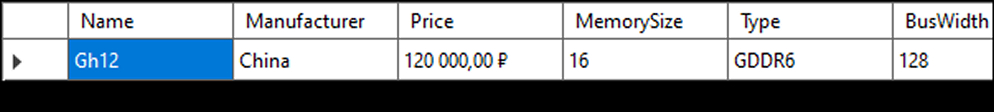
\includegraphics[width=0.8\textwidth]{fig/image 62.jpg} % Placeholder
	\caption{Форматирование столбца \texttt{Price}}
	\label{fig:6.13}
\end{figure}

\begin{code}
	\inputminted[firstline = 202, lastline=217]{csharp}{../2lab/WinFormsApp1example_/Form1.cs}
	\caption{\colorGIT{\href{https://github.com/WebMasterIT/Csharp_Labs/blob/c79e983c4cab3c416e44b6d5f9854b292fdeae26/2lab/WinFormsApp1example_/Form1.cs\#L202-L217}{Метод}} форматирования строки со стоимостью}
	\label{list:6.14}
\end{code}

А затем вызывать этот метод у каждой таблицы (свойство \texttt{CellFormatting}) (Листинг \ref{list:6.15}).

\begin{code}
	\inputminted[firstline = 219, lastline=232]{csharp}{../2lab/WinFormsApp1example_/Form1.cs}
	\caption{Вызов \colorGIT{\href{https://github.com/WebMasterIT/Csharp_Labs/blob/c79e983c4cab3c416e44b6d5f9854b292fdeae26/2lab/WinFormsApp1example_/Form1.cs\#L219-L232}{метода}} форматирования}
	\label{list:6.15}
\end{code}

\clearpage
\section{Интерфейс приложения}
Далее представлены примеры интерфейса приложения.
Добавление данных в таблицу \texttt{Components} представлено на рисунке \ref{fig:6.16}.

\begin{figure}[H]
	\centering
	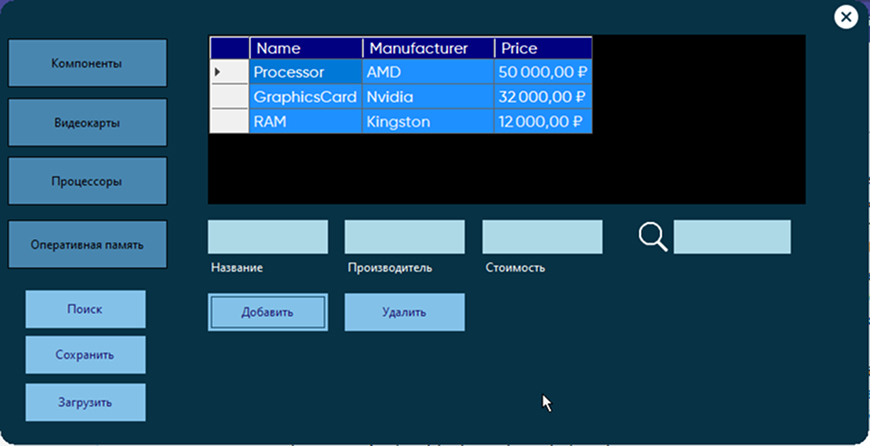
\includegraphics[width=0.8\textwidth]{fig/image 69.jpg} % Placeholder
	\caption{Добавление данных в таблицу компонентов}
	\label{fig:6.16}
\end{figure}

Удаление осуществляется нажатием на соответствующую строку и затем нажатием кнопки <<Удалить>> (Рисунок \ref{fig:6.17}).

\begin{figure}[H]
	\centering
	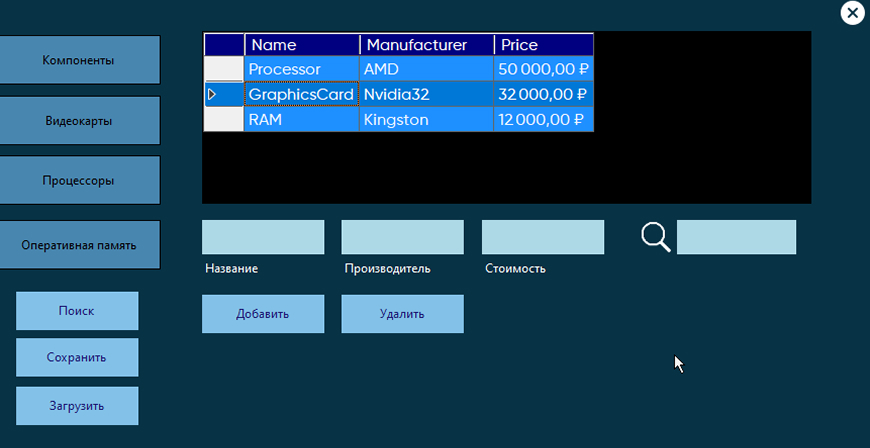
\includegraphics[width=0.8\textwidth]{fig/image 70.jpg} % Placeholder
	\caption{Удаление данных из таблицы компонентов}
	\label{fig:6.17}
\end{figure}

\clearpage
Поиск осуществляется путем ввода данных в поле поиска и нажатием кнопки <<Поиск>>. Поля поиска в данном случае уникальные для каждой панели (класса), но кнопка поиска одна (Рисунок \ref{fig:6.18}).

\begin{figure}[H]
	\centering
	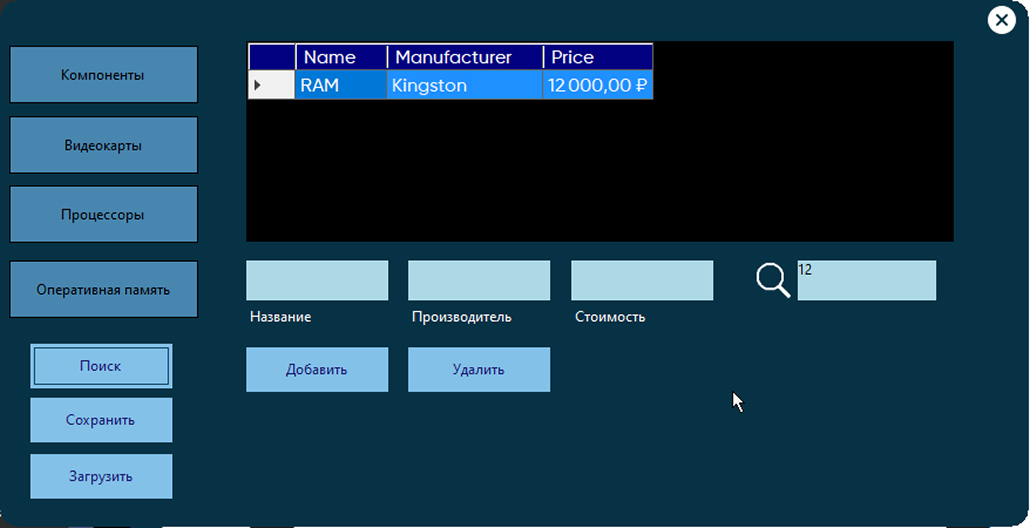
\includegraphics[width=0.8\textwidth]{fig/image 72.jpg} % Placeholder
	\caption{Поиск данных в таблице компонентов}
	\label{fig:6.18}
\end{figure}

Поиск осуществляется путем ввода данных в поле поиска и нажатием кнопки <<Поиск>>. Поля поиска в данном случае уникальные для каждой панели (класса), но кнопка поиска одна (Рисунок \ref{fig:6.19}).

\begin{figure}[H]
	\centering
	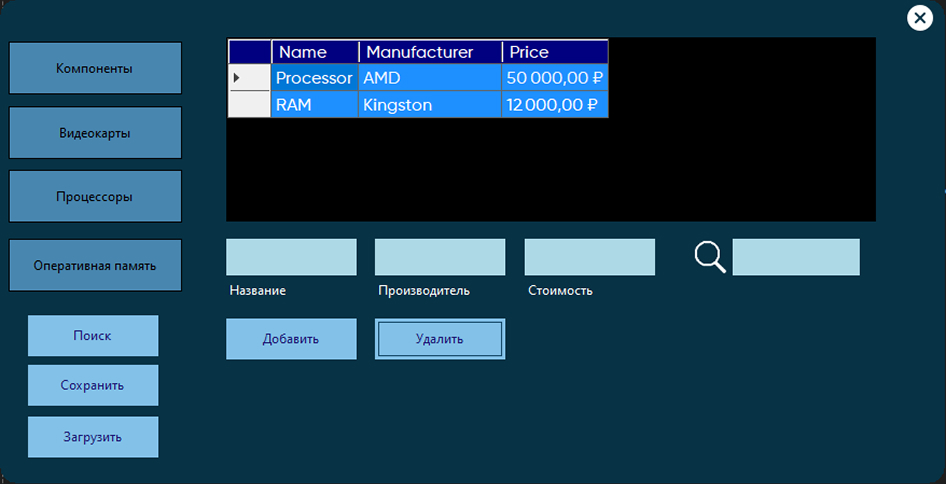
\includegraphics[width=0.8\textwidth]{fig/image 71.jpg} % Placeholder
	\caption{Поиск данных в таблице компонентов (пример с результатом)}
	\label{fig:6.19}
\end{figure}

\newpage

\noindent Также реализовано добавление данных в таблицы других классов (Рисунок \ref{fig:6.20}).

\begin{figure}[H]
	\centering
	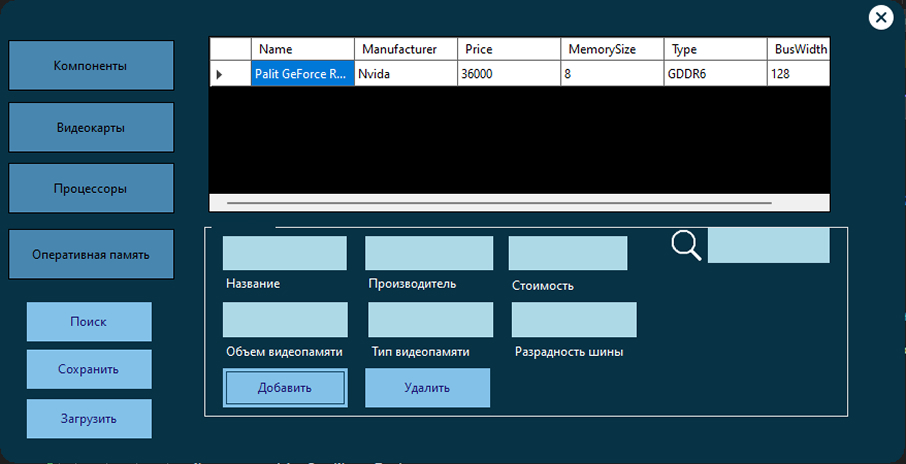
\includegraphics[width=0.8\textwidth]{fig/image 73.jpg} % Placeholder
	\caption{Добавление данных в таблицу видеокарт}
	\label{fig:6.20}
\end{figure}
\end{document}
